\documentclass[aspectratio=169]{beamer}

\usetheme{metropolis}

\usefonttheme{professionalfonts}
\usepackage[familydefault,light]{Chivo}

\usepackage{lmodern}
\usepackage[english]{babel}

\usepackage{fontspec}
\defaultfontfeatures{Ligatures=TeX}

\usepackage{multicol}

\usepackage{listings}

\usepackage{datetime}
\setdefaultdate{\usdate}

\usepackage{graphicx}
\graphicspath{{assets/}}

\newcommand{\german}[1]{{#1}}

\title{Low-Code vs.\texorpdfstring{\\}{} Model-Driven Architecture}
\author{Markus Reiter}


\date{\formatdate{12}{01}{2021}}

\institute{supervised by Prof. Dr. Ruth Breu}

\begin{document}
  \maketitle

  \begin{frame}{Outline}
    \begin{itemize}
      \item Motivation
      \item Model-Driven Architecture
      \item Low-Code Architecture
      \item Criticisms
      \item Evaluation of Low-Code Tools
      \item Findings \& Future Work
      \item Conclusion
    \end{itemize}
  \end{frame}

  \begin{frame}{Motivation}
    \begin{itemize}
      \item What are the advantages and disadvantages of low-code tools do?
      \item Are they a viable alternative to model-driven or traditional development?
      \item When to choose one approach over the other?
    \end{itemize}
  \end{frame}

  \begin{frame}{Model-Driven Architecture}
    \begin{itemize}
      \item provides a set of guidelines for the structuring of specifications
      \item standardise on models in a given domain to reduce code duplication and speed up development
      \item code (fully or partially) generated from models, e.g. from UML diagrams
      \item aimed at developers who have good understanding of underlying programming languages
    \end{itemize}
  \end{frame}

  \begin{frame}{Model-Driven Architecture}
    \begin{itemize}
      \item Example: Swagger
        \begin{itemize}
          \item API specification given in OpenAPI format
          \item API client is generated for the specified programming language
          \item support for new languages/frameworks can be added by implementing a new generator
          \item very easy to provide clients for many languages with virtually no development effort
        \end{itemize}
    \end{itemize}
  \end{frame}

  \begin{frame}{Low-Code Architecture}
    \begin{itemize}
      \item provides pre-built application components
      \item graphical user interface for creating both the
            application logic as well as the user interface
      \item typically aimed at end-users rather than developers
    \end{itemize}
  \end{frame}

  \begin{frame}{Criticisms}
    \begin{itemize}
      \item Model-Driven Architecture
        \begin{itemize}
          \item UML diagrams lack details included in the code itself.
          \item “the Code is the design” - Should models be derived from code instead of code from models?
        \end{itemize}
      \item Low-Code Architecture
        \begin{itemize}
          \item Unsuitable for implementing scalable and mission-critical applications.
          \item Increase in unsupported applications built by shadow IT,
                i.e. applications which are not controlled by a company's IT department.
        \end{itemize}
      \item Do these approaches actually make development easier and cheaper?
    \end{itemize}
  \end{frame}

  \begin{frame}{Evaluation of Low-Code Tools}
    \begin{itemize}
      \item Find low-code tools in the following categories:
          \begin{itemize}
            \item open-source
            \item developed by well-known company
            \item developed by unknown company
            \item old/well-established platform
            \item new/unestablished
          \end{itemize}
      \item Set up each tool
      \item Build a test application (TODO List) with each tool
    \end{itemize}
  \end{frame}

  \begin{frame}{Open Standard Business Platform (OSBP)}
    \begin{itemize}
      \item open-source
      \item plug-in for the Eclipse IDE developed since 2016
      \item community version of the commercial OS.bee product \\
            developed by COMPEX
      \item latest version over one year old
      \item does not work with latest version of the Eclipse IDE
    \end{itemize}
  \end{frame}

  \begin{frame}{Corteza Low Code}
    \begin{itemize}
      \item open-source
      \item part of the Corteza Project initiated by Crust Technology in 2019
      \item the Corteza Project includes a CRM solution built on top of Corteza~Low~Code, among other things
      \item web-based platform
      \item test by signing up with a GitHub or Google account or \\
            by deploying it locally using Docker
    \end{itemize}
  \end{frame}

  \begin{frame}{Corteza Low Code}
    \begin{itemize}
      \item made for building record-based management applications
      \item process for building the test application:
        \begin{enumerate}
          \item create application namespace
          \item create module for TODO List records, specifying the necessary fields (status, title, body)
          \item create page and add a list block linked to the module
        \end{enumerate}
    \end{itemize}
  \end{frame}

  \begin{frame}[standout]{Corteza Low Code: Editor}
    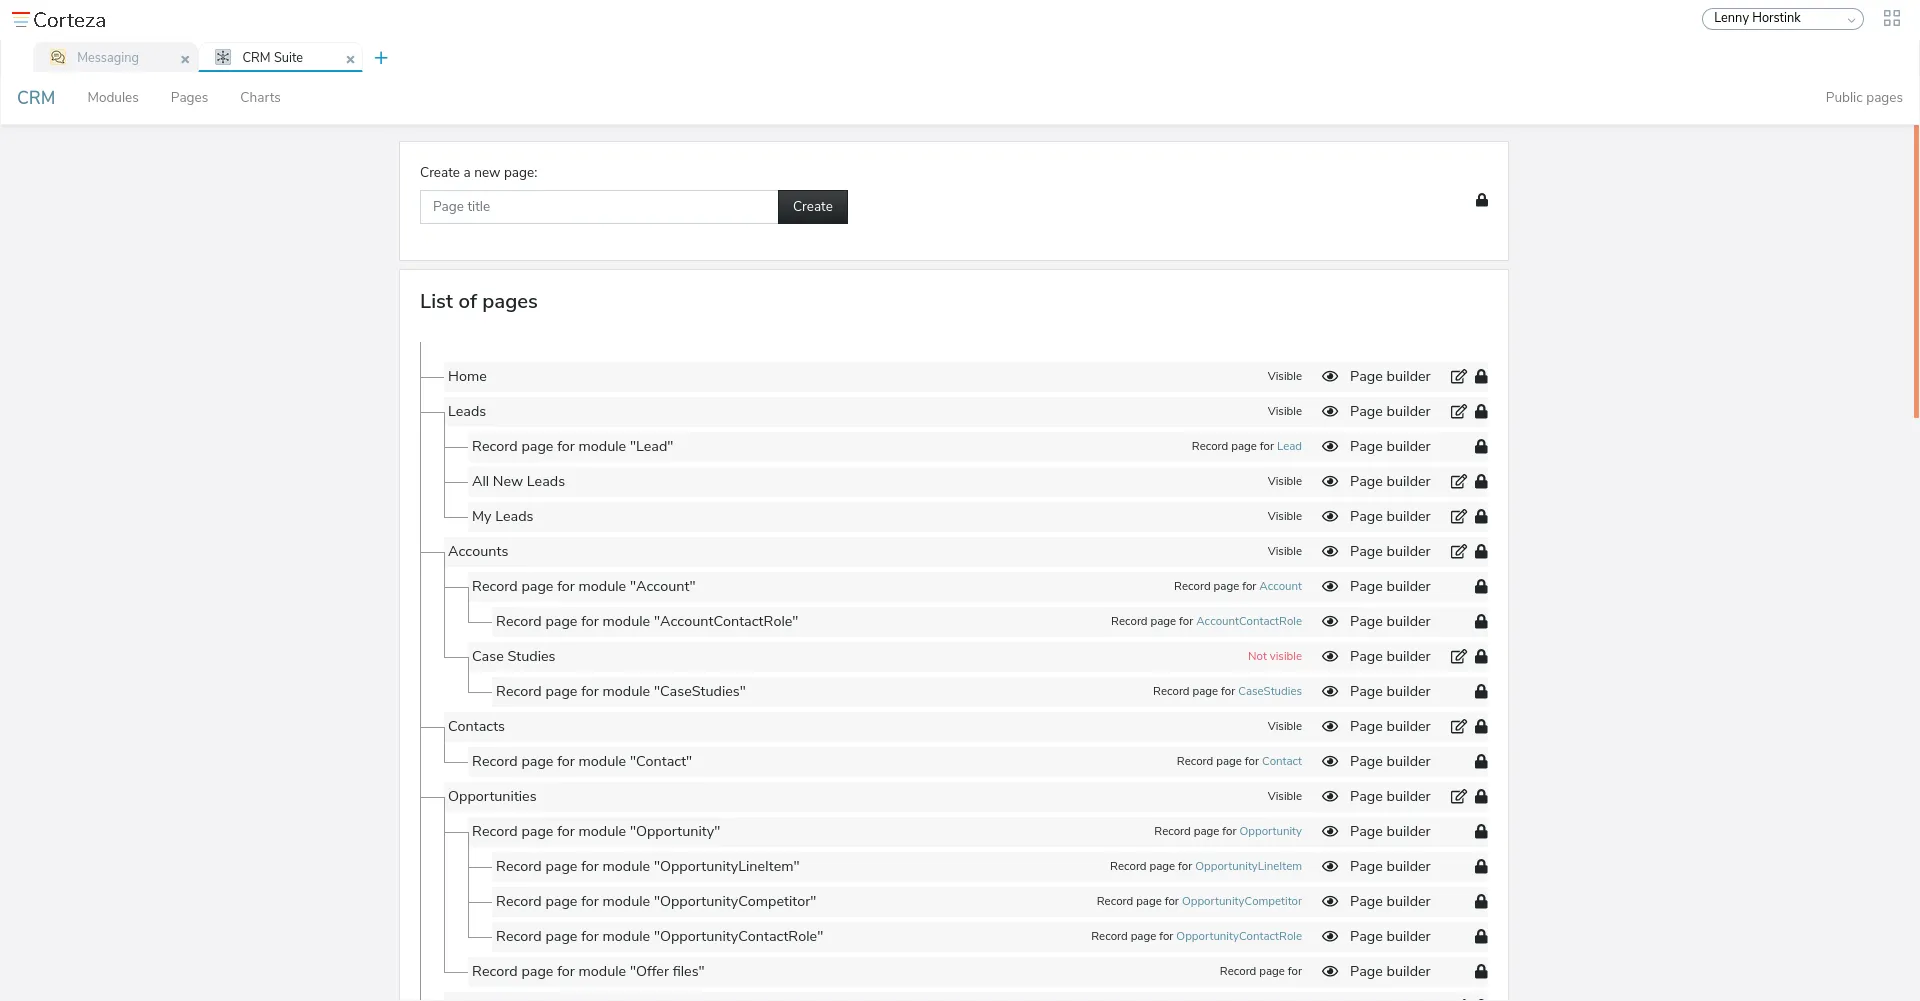
\includegraphics[width=\textwidth]{corteza-low-code-pages}
  \end{frame}

  \begin{frame}[standout]{Corteza Low Code: Application}
    \begin{figure}
      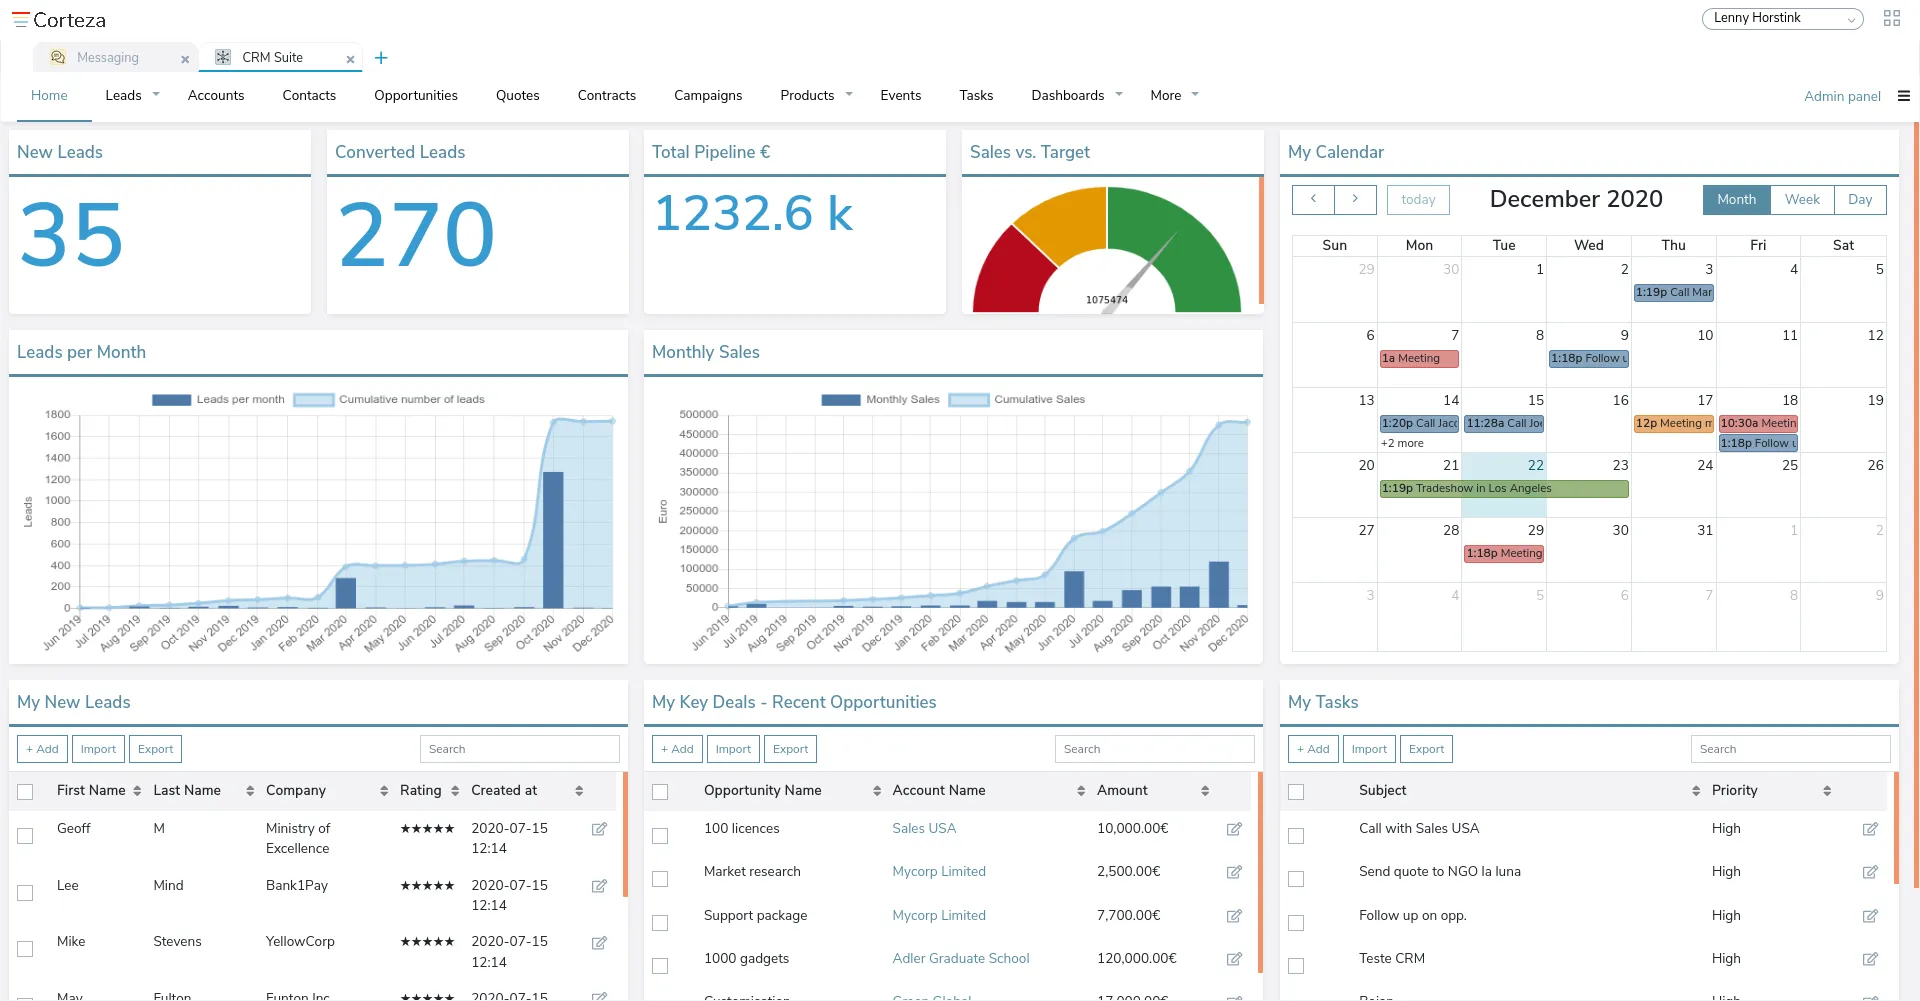
\includegraphics[width=\textwidth]{corteza-low-code-crm-home}
    \end{figure}
  \end{frame}

  \begin{frame}{Oracle APEX (Application Express)}
    \begin{itemize}
      \item commercial
      \item initially released as Oracle Flows in 2000
      \item web-based platform
      \item test by signing up for an Oracle Cloud account or \\
            by requesting an APEX workspace
    \end{itemize}
  \end{frame}

  \begin{frame}{Oracle APEX (Application Express)}
    \begin{itemize}
      \item process for building the test application:
        \begin{enumerate}
          \item create database table for TODO List items \\
                (requires basic SQL knowledge)
          \item create new blank application
          \item add list view to home page and select \\
                the corresponding database table
          \item add new form page (dialog style) and select \\
                the corresponding database table
          \item add a button to the home page that opens the form page
          \item add a dynamic action that refreshes the list view \\
                when the form dialog is closed
        \end{enumerate}
    \end{itemize}
  \end{frame}

  \begin{frame}[standout]{Oracle APEX: Page Designer}
    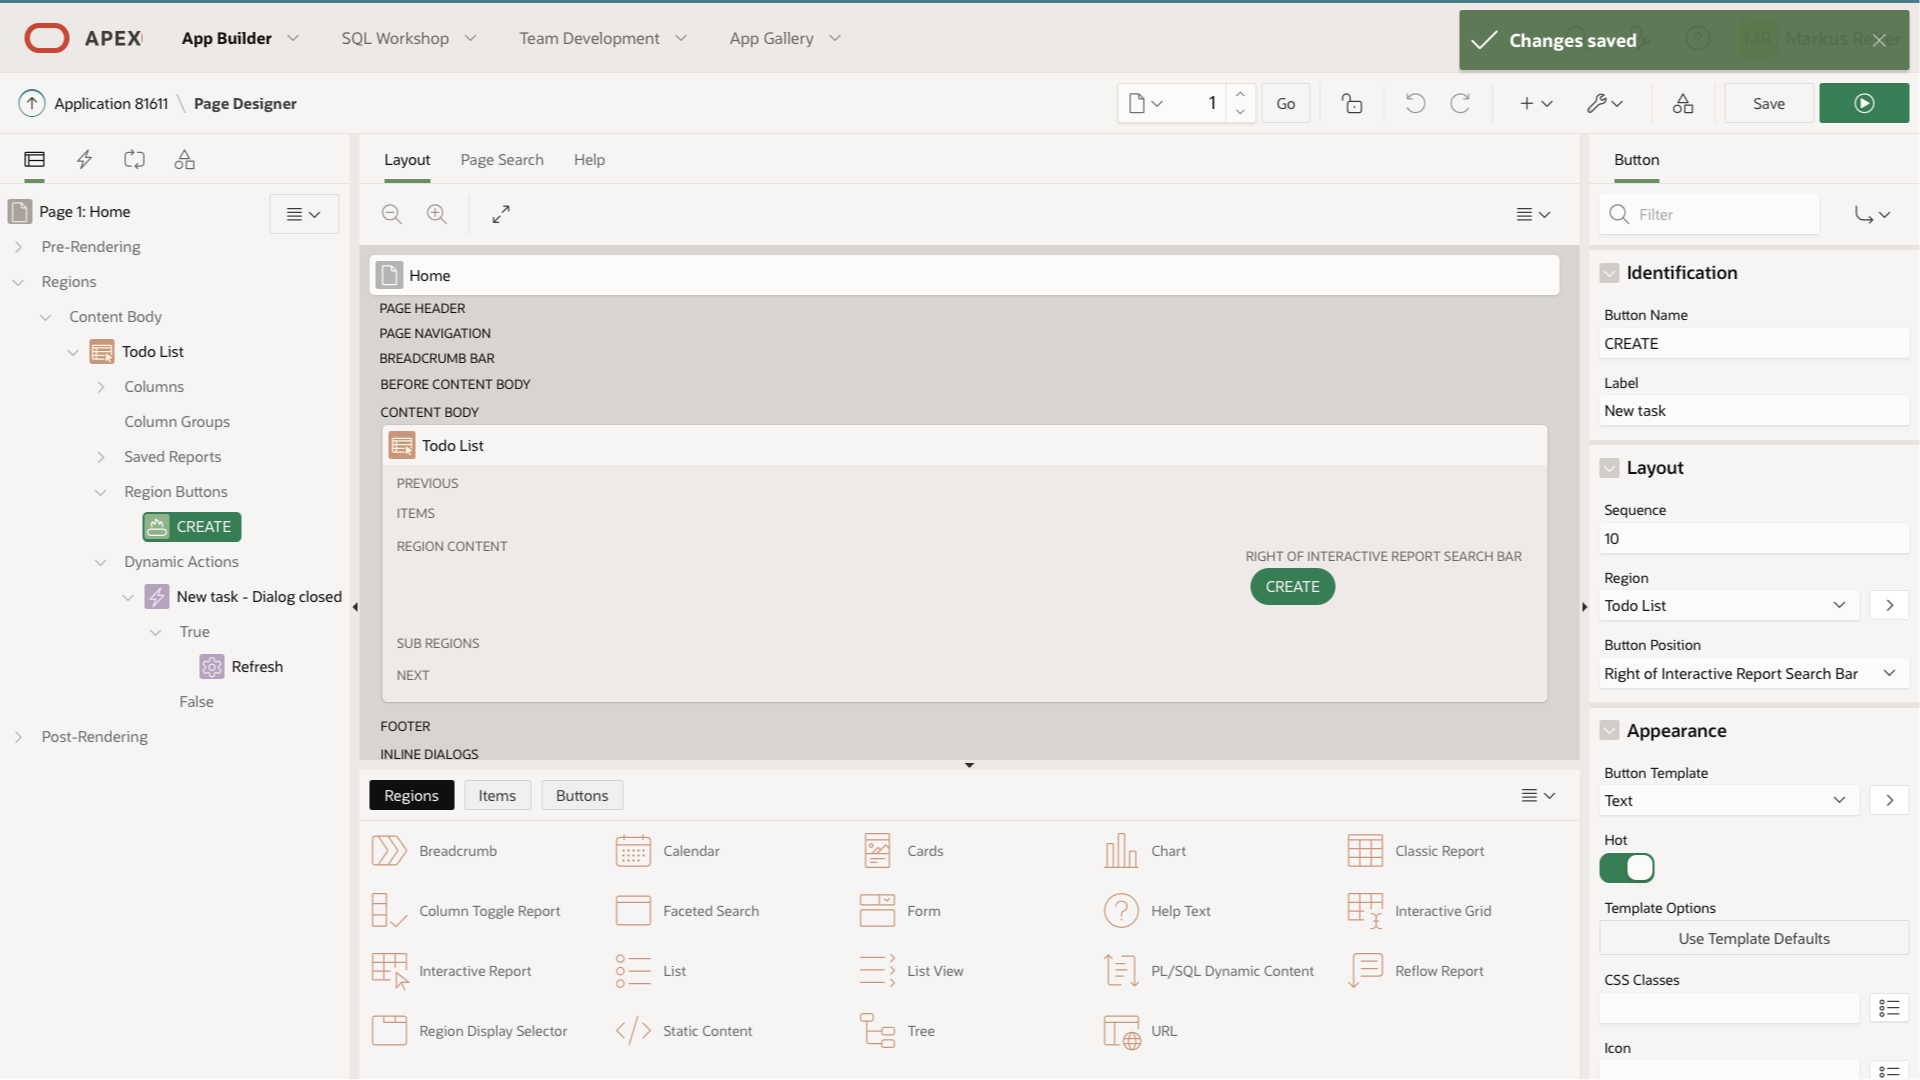
\includegraphics[width=\textwidth]{oracle-apex-page-designer}
  \end{frame}

  \begin{frame}[standout]{Oracle APEX: Application}
    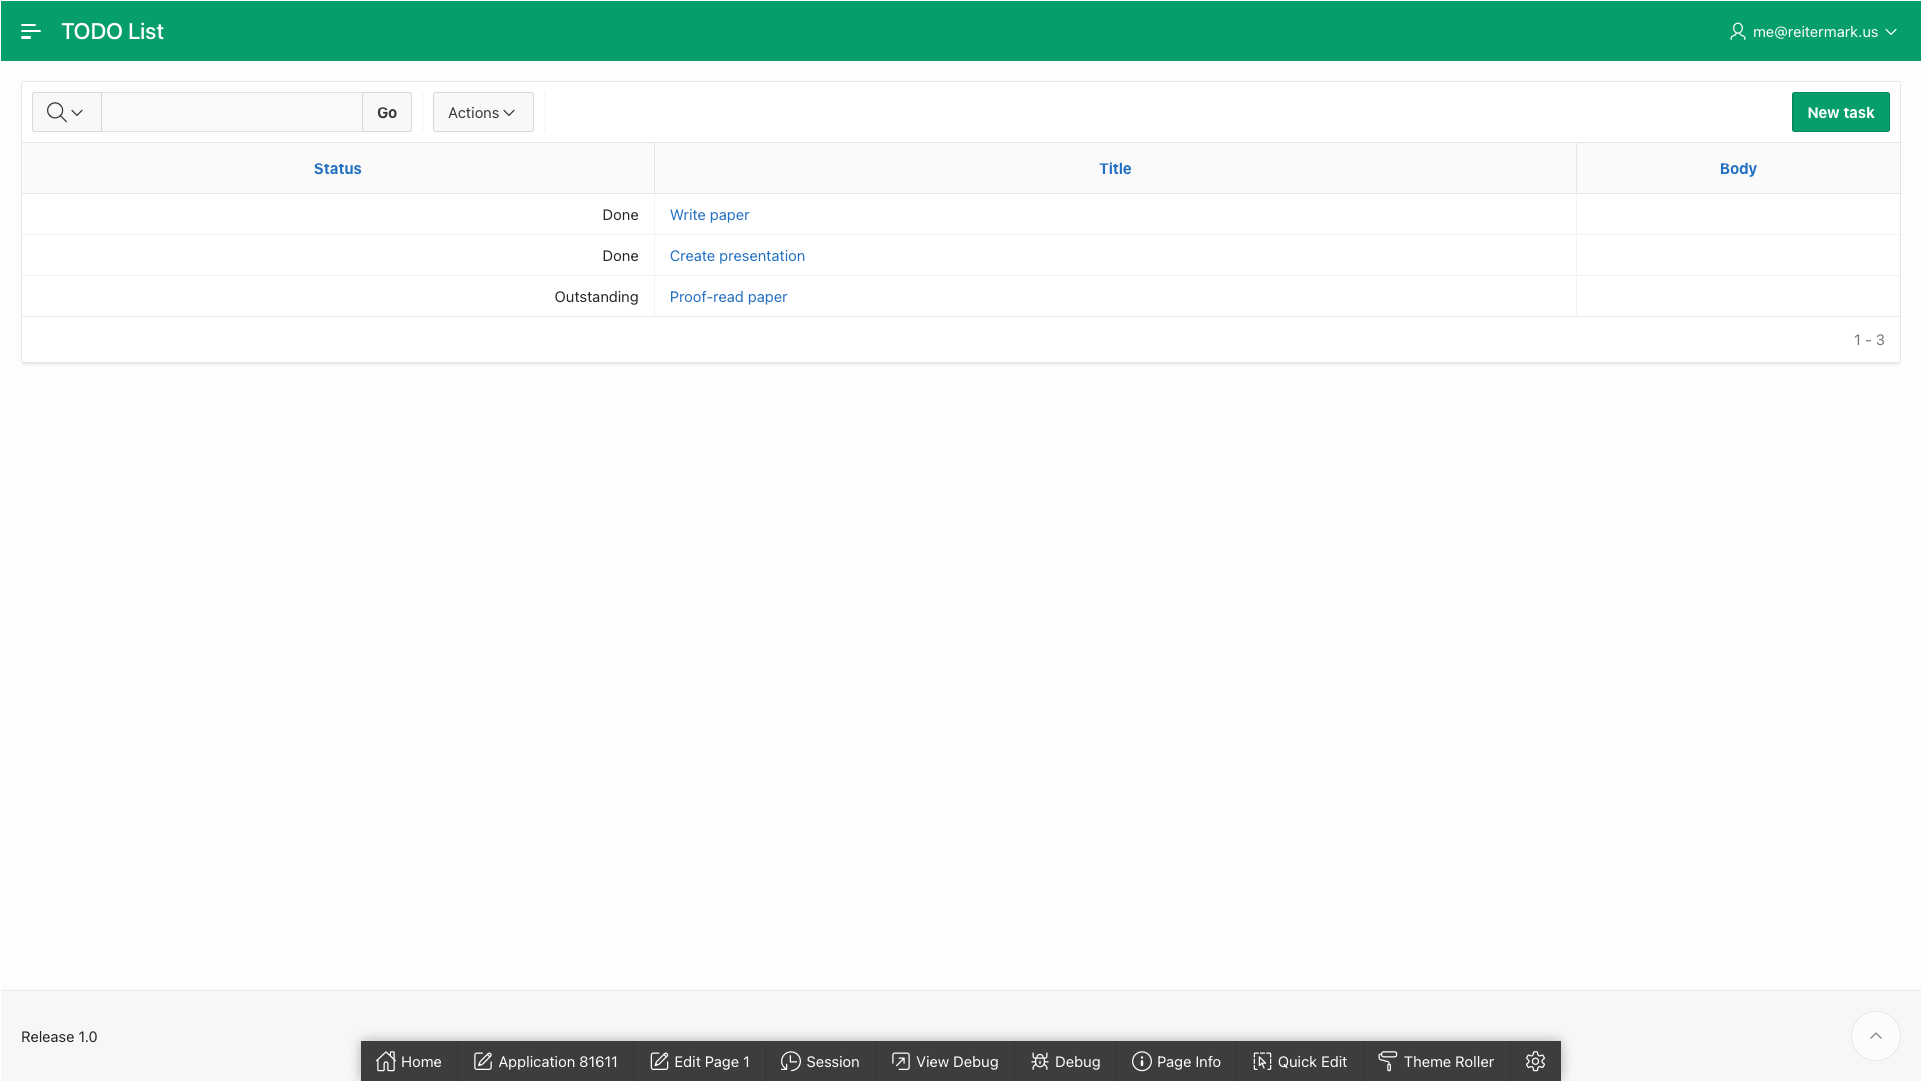
\includegraphics[width=\textwidth]{oracle-apex-todo-list-application}
  \end{frame}

  \begin{frame}{Simplifier}
    \begin{itemize}
      \item commercial
      \item initially released by iTiZZiMO in 2012
      \item web-based platform
      \item test by using the Simplifier Playground (data is wiped every day) or \\
            by requesting a Simplifier test instance
    \end{itemize}
  \end{frame}

  \begin{frame}{Simplifier}
    \begin{itemize}
      \item process for building the test application:
        \begin{enumerate}
          \item create database connector (SQLite)
          \item create database schema for TODO List items and deploy to connector
          \item add list view and button to home page
          \item add new page containing a form with input fields and button
          \item create processes for
            \begin{itemize}
              \item loading items into list view
              \item submitting the form page
              \item opening the form page with the button
            \end{itemize}
        \end{enumerate}
    \end{itemize}
  \end{frame}

  \begin{frame}[standout]{Simplifier: Process}
    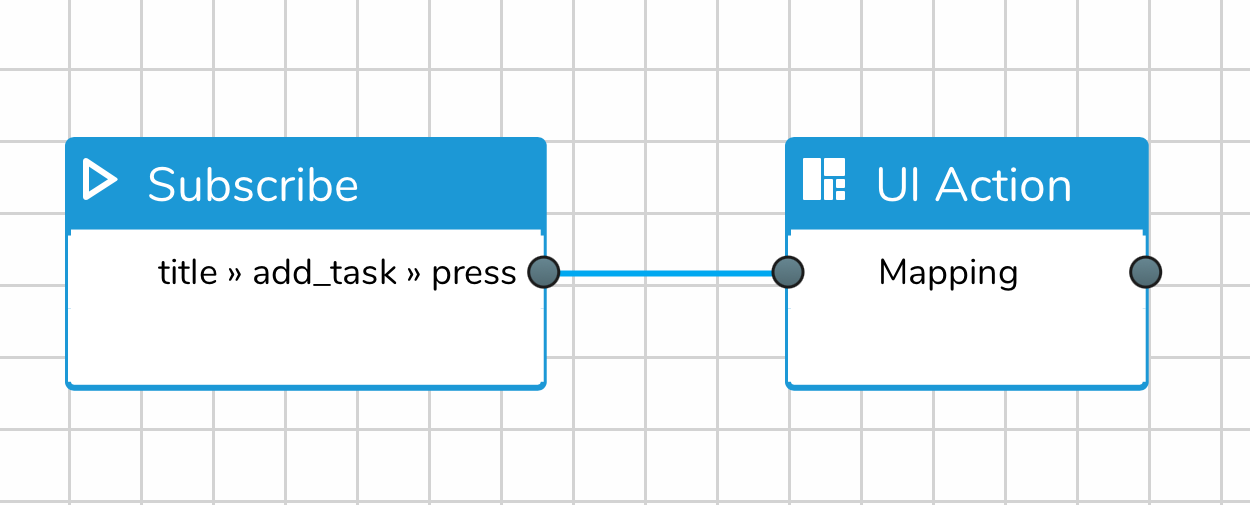
\includegraphics[width=\textwidth]{simplifier-story-overview}
  \end{frame}

  \begin{frame}[standout]{Simplifier: Process}
    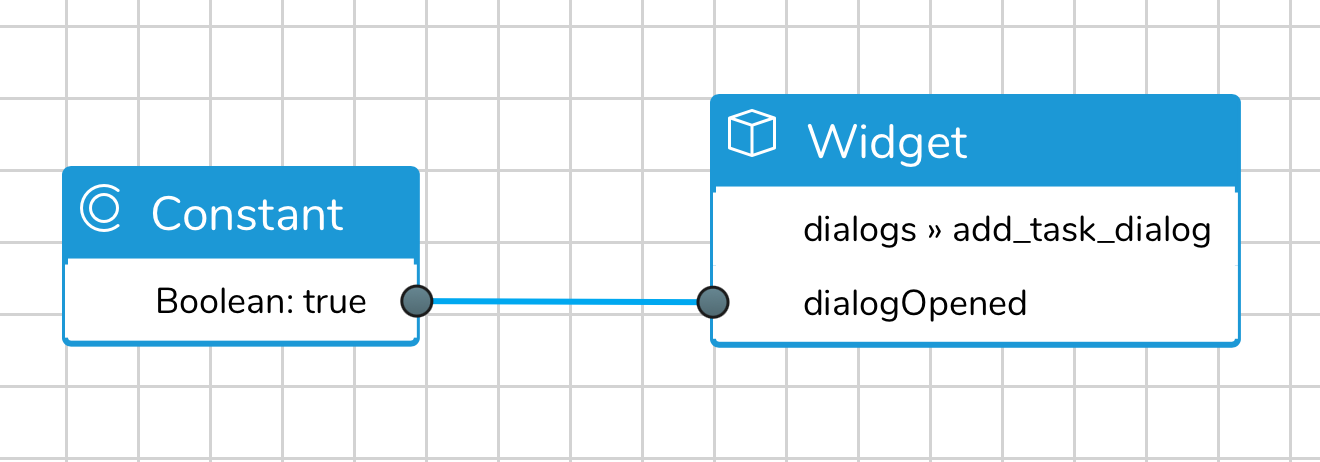
\includegraphics[width=\textwidth]{simplifier-story-ui-action}
  \end{frame}

  \begin{frame}[standout]{Simplifier: Application Editor}
    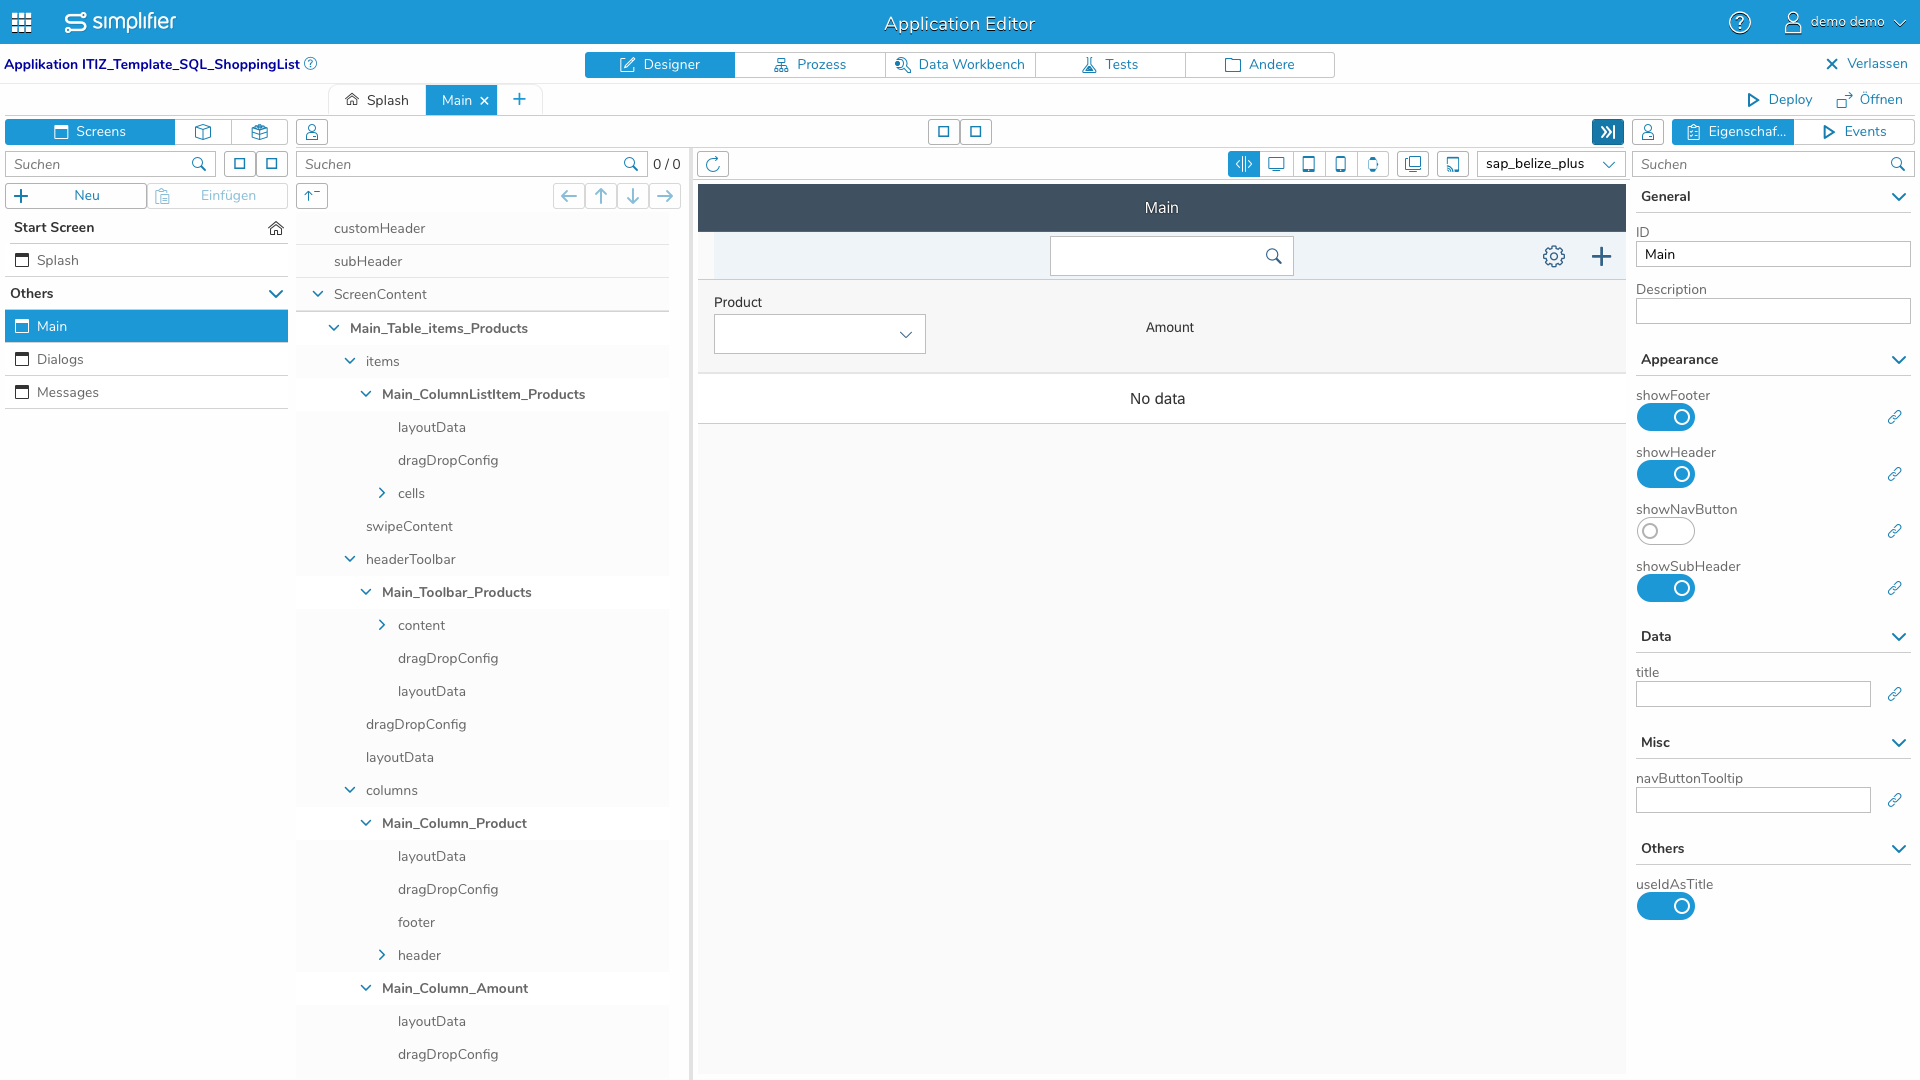
\includegraphics[width=\textwidth]{simplifier-application-editor}
  \end{frame}

  \begin{frame}[standout]{Simplifier: Application}
    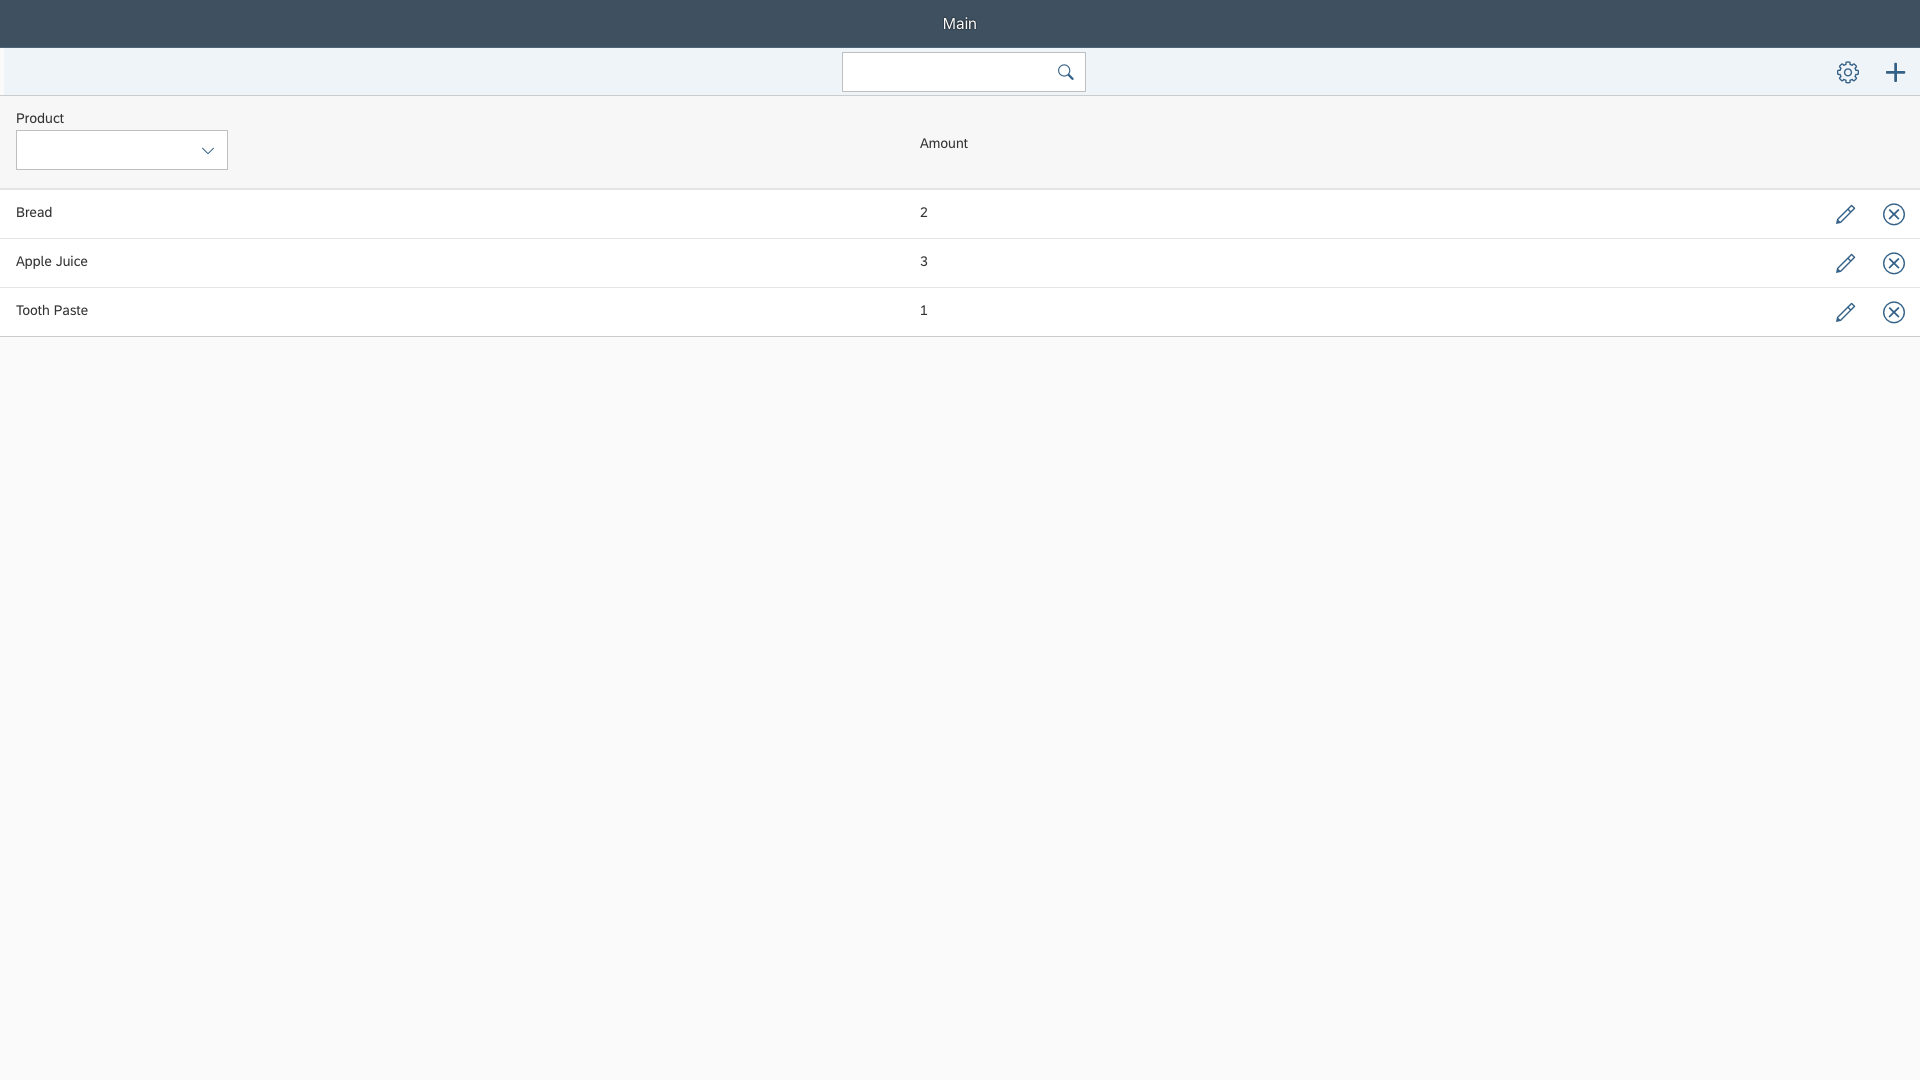
\includegraphics[width=\textwidth]{simplifier-shopping-list-application}
  \end{frame}

  \begin{frame}{Mendix}
    \begin{itemize}
      \item commercial
      \item founded in 2005 as a subsidiary of Siemens
      \item web-based platform (Mendix Studio) and Windows application \\
            (Mendix Studio Pro) with advanced features
      \item test by signing up for a regular account which allows hosting unlimited applications (with 1GB of memory and 0.5GB of storage per application)
    \end{itemize}
  \end{frame}

  \begin{frame}{Mendix}
    \begin{itemize}
      \item process for building the test application:
        \begin{enumerate}
          \item create blank application
          \item add list view and button to home page, which prompts the user to select or create a new data source
          \item create data source for TODO List items
          \item add new form page linked to the corresponding data source
          \item add button to home page that opens the form page
        \end{enumerate}
    \end{itemize}
  \end{frame}

  \begin{frame}[standout]{Mendix Studio}
    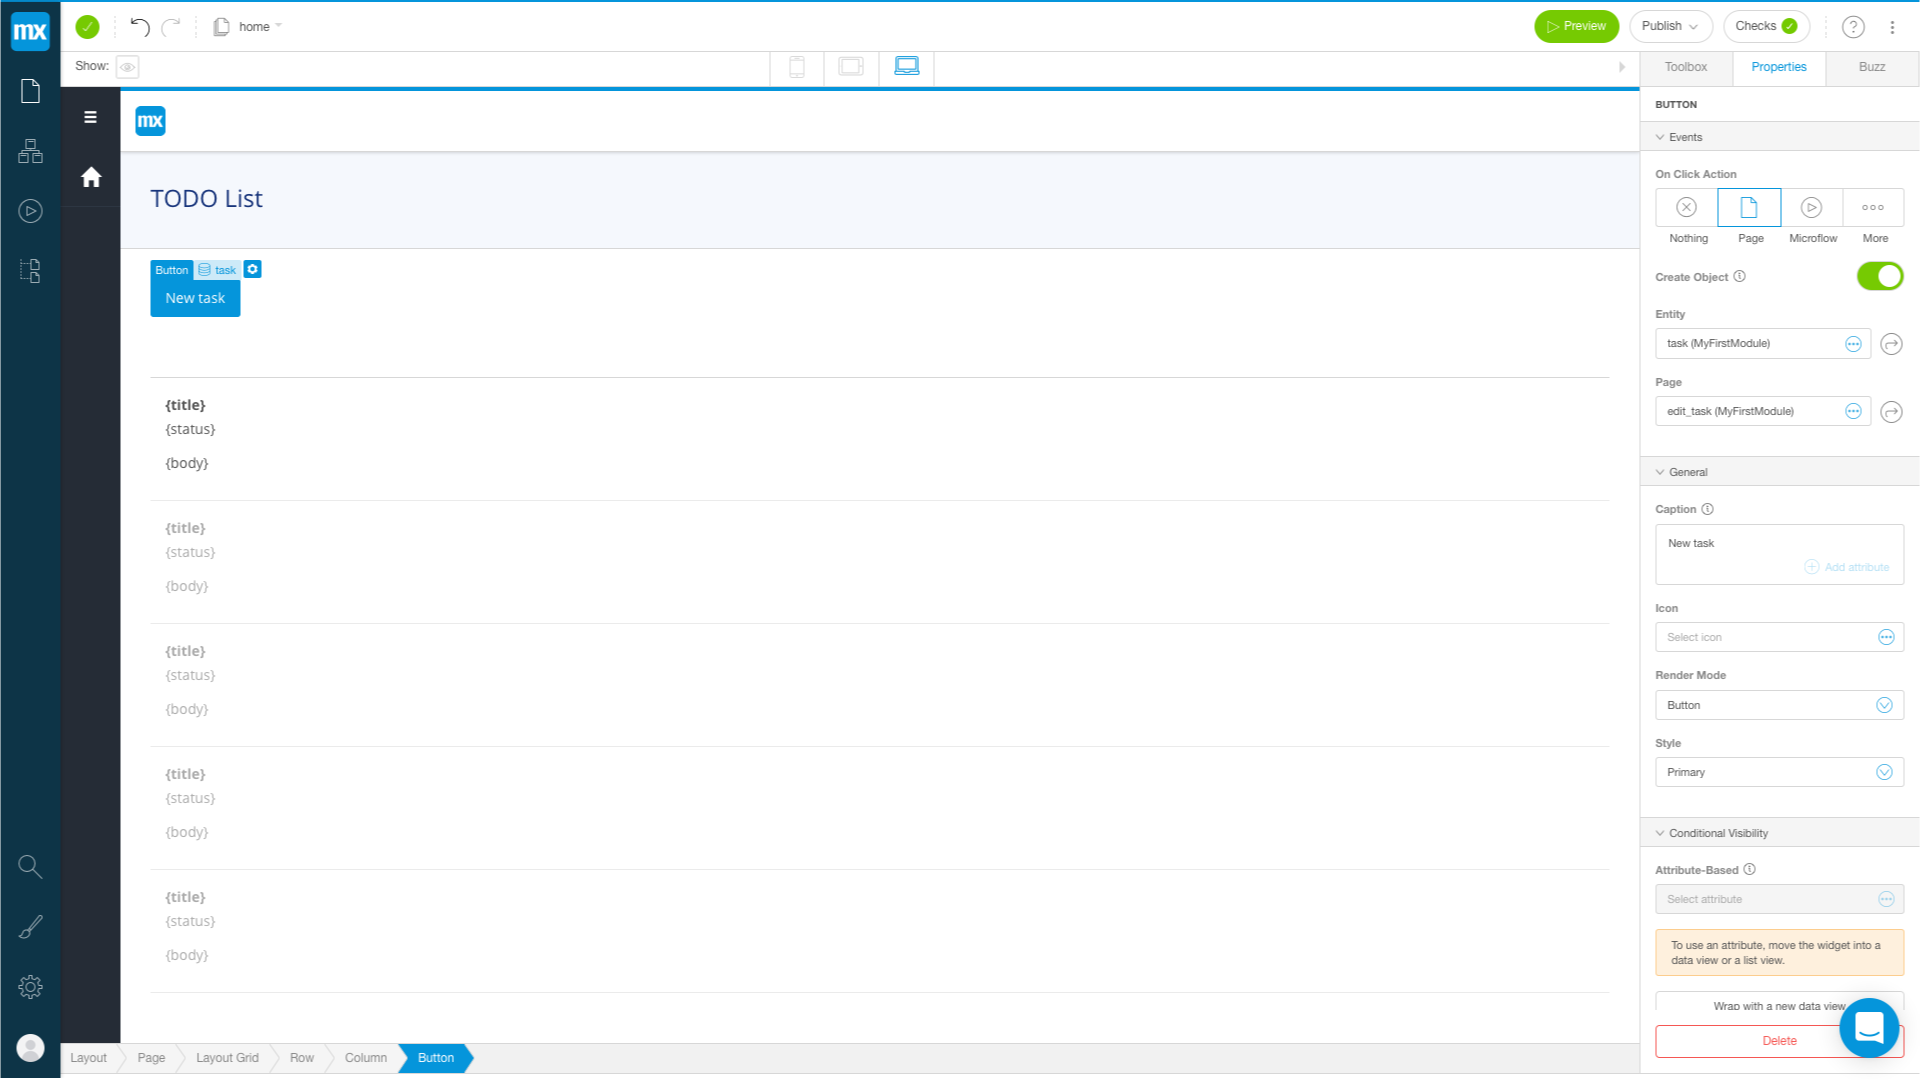
\includegraphics[width=\textwidth]{mendix-studio}
  \end{frame}

  \begin{frame}[standout]{Mendix: Application}
    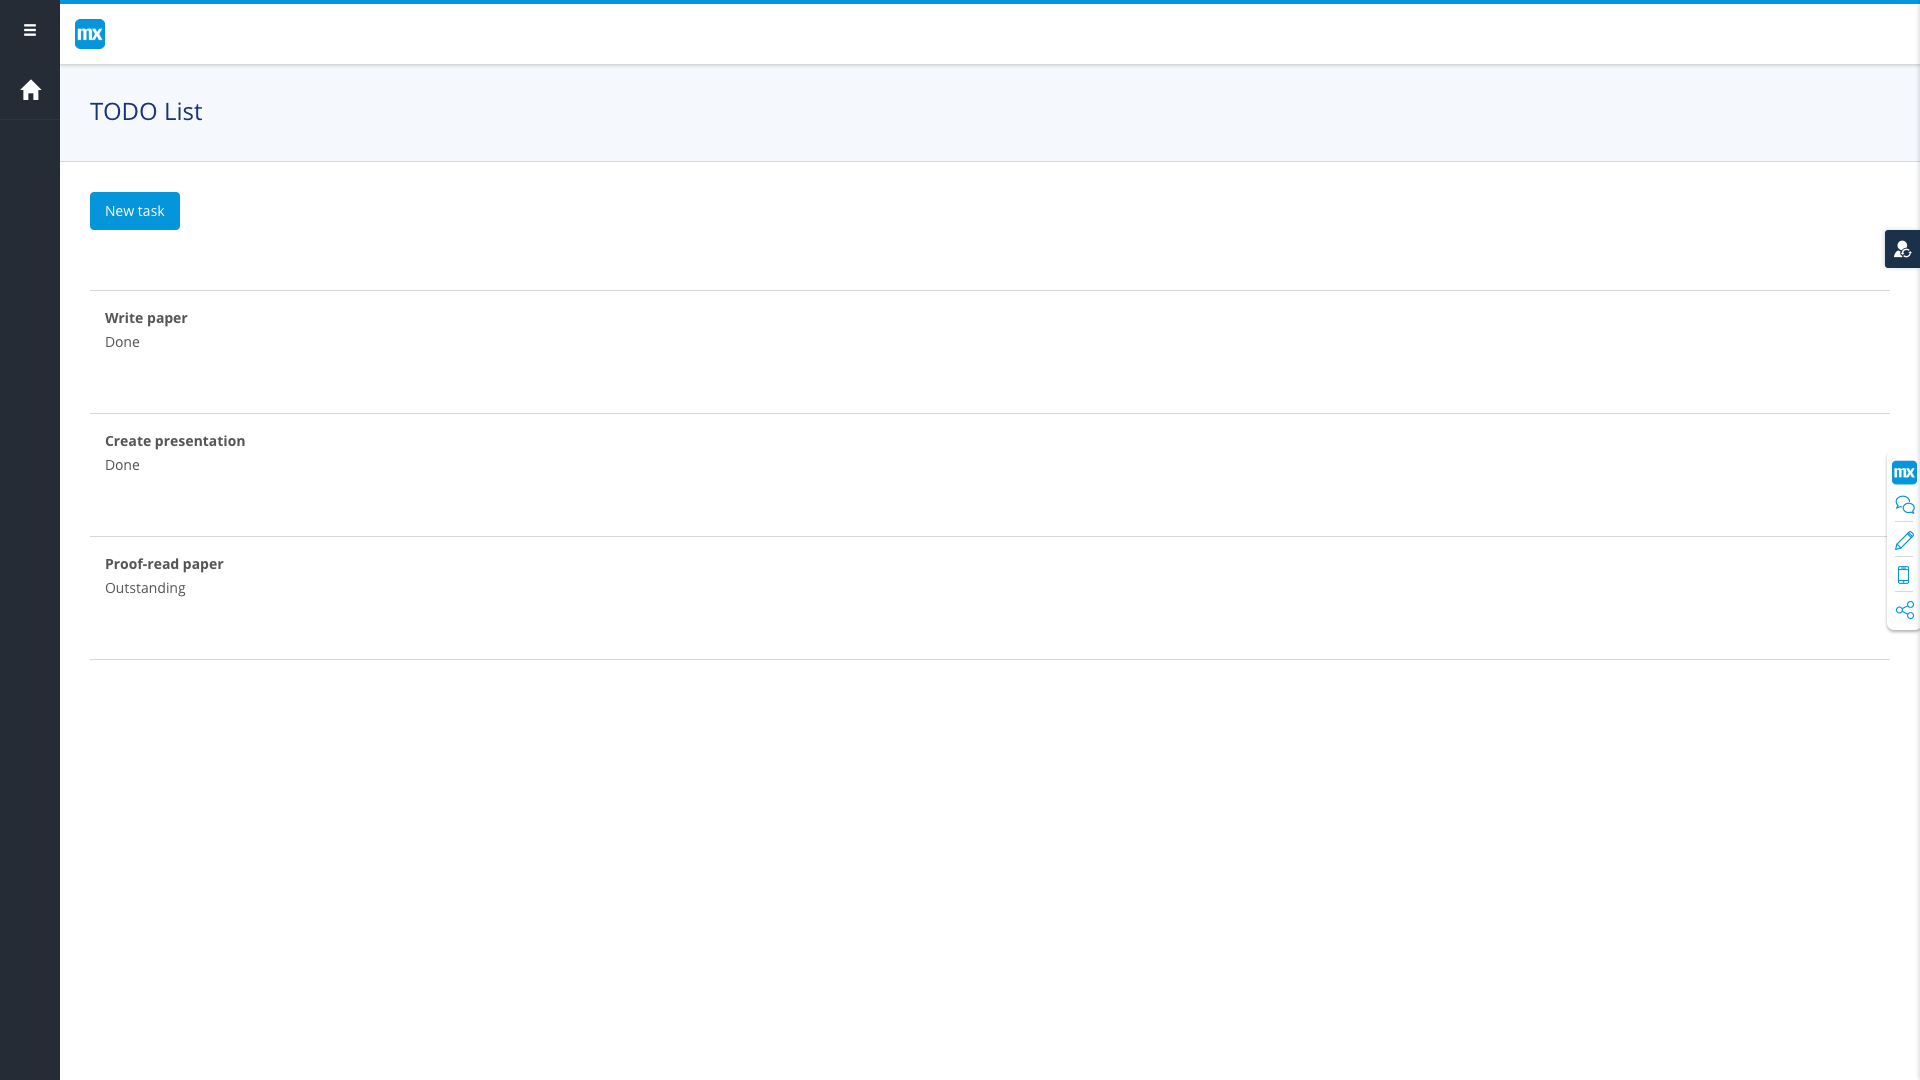
\includegraphics[width=\textwidth]{mendix-todo-list-application}
  \end{frame}

  \begin{frame}{Unique Features}
    \begin{itemize}
      \item \textbf{Oracle APEX}
        \begin{itemize}
          \item Creation of applications from existing data, e.g. CSV files
        \end{itemize}
      \item \textbf{Mendix}
        \begin{itemize}
          \item AI-assisted wizard for creating custom workflows (microflows)
          \item publishing as native mobile applications for iOS and Android
        \end{itemize}
    \end{itemize}
  \end{frame}

  \begin{frame}{Assessment of Low-Code Tools}
    \begin{itemize}
      \item ease of use
      \item customisability
      \item portability
      \item scalability
      \item suitability for mission-critical applications
    \end{itemize}
  \end{frame}

  \begin{frame}{Assessment of Low-Code Tools}
    \begin{table}[]
    \begin{tabular}{l|l|l|l|l|l|}
    \cline{2-6}
                                           & \textbf{OSBP} & \textbf{Corteza} & \textbf{APEX}   & \textbf{Simplifier} & \textbf{Mendix} \\ \hline
    \multicolumn{1}{|l|}{ease of use}      & N/A  & high    & medium & medium     & high   \\ \hline
    \multicolumn{1}{|l|}{customisability}  & N/A  & low     & medium & medium     & high   \\ \hline
    \multicolumn{1}{|l|}{portability}      & N/A  & medium  & low    & medium     & medium \\ \hline
    \multicolumn{1}{|l|}{scalability}      & N/A  & medium\footnote{medium in general, high for certain types of applications, e.g. management applications} & high   & high       & high   \\ \hline
    \multicolumn{1}{|l|}{mission-criticality} & low  & high    & high   & medium\footnote{medium only due to the problems encountered, high otherwise}    & high   \\ \hline
    \end{tabular}
    \end{table}
  \end{frame}

  \begin{frame}{Findings \& Future Work}
    \begin{itemize}
      \item very small number of open-source low-code tools
        \begin{itemize}
          \item assumption: open-source community mostly consists of developers, so there is no need/demand for low-code platforms
          \item future work: investigate low-code other types of platforms and compare their presence in the open-source vs. the commercial space
        \end{itemize}
      \item more streamlined user interface in the more mature products like Oracle APEX and Mendix
      \item lack of portability is a valid concern for low-code tools, \\
            stored data may be the only element of a platform that is portable by using
    \end{itemize}
  \end{frame}

  \begin{frame}{Conclusion}
    \begin{itemize}
      \item low-code platforms are a valid alternative to model-driven development
      \item low-code platforms are not as flexible and limited in the ways they can be extended
      \item choice between low-code and model-driven architecture:
        \begin{itemize}
          \item highly dependent on which low-code platform is used, \\
                similar to choosing a programming language or framework for a particular task
          \item highly dependent on the application requirements, \\
                low-code well-suited for management applications (e.g. process management, CRM)
        \end{itemize}
    \end{itemize}
  \end{frame}


  \begin{frame}[standout]
    Questions?
  \end{frame}
\end{document}
